% id: 0637
% book: RPM 중학 3-2 · 07 상자그림과 산점도
% section: 유형 07 산점도의 이해 (2)
% figure: crop:fig-0637.png
% answer: ③
% answer_source: 답지
% variant_level: 0 (원본 전사)
% 이 파일은 build.mjs 가 items.json 에서 만든다. 고칠 때는 items.json 을 고친다.
\smash{\raisebox{1.5mm}{\dmkichul{RPM 중학 3-2 0637번 · 109쪽 · 대표문제}}}
\noindent\begin{minipage}[t]{0.58\linewidth}\vspace{0pt}\raggedright 오른쪽 그림은 효상이네 반 학생 24명이 지난달과 이번 달에 도서관을 방문한 횟수를 조사하여 나타낸 산점도이다. 지난달과 이번 달에 도서관을 방문한 횟수의 합이 15회 이상인 학생은 몇 명인가?\end{minipage}\hfill\begin{minipage}[t]{0.4\linewidth}\vspace{0pt}\centering \setlength{\dmfigw}{90.4pt}\ifdim\dmfigw>\linewidth\setlength{\dmfigw}{\linewidth}\fi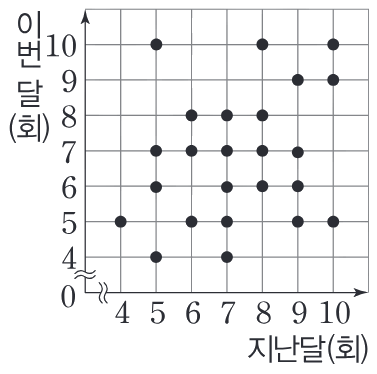
\includegraphics[width=\dmfigw]{figures/fig-0637.png}\end{minipage}\par
\begin{choices32}{9명}{10명}{11명}{12명}{13명}\end{choices32}
